\section{Design}

\subsection{High Level Overview}

The system will comprise 3 parts required to simulate and program a proprietary processor. It will include a virtual machine to emulate the execution of binary machine code catridges, an assembler to translate higher level assembly code into machine code, and finally a compiler for a higher level language to easily program complex applications to run on the processor.

The virtual machine consists of two main processes, the debugger and interpreter. The interpreter will continiously step through memory, decoding and executing instructions sequentially whilst displaying the contents of VRAM through the pixel display.

\bigskip

\shadowbox{
    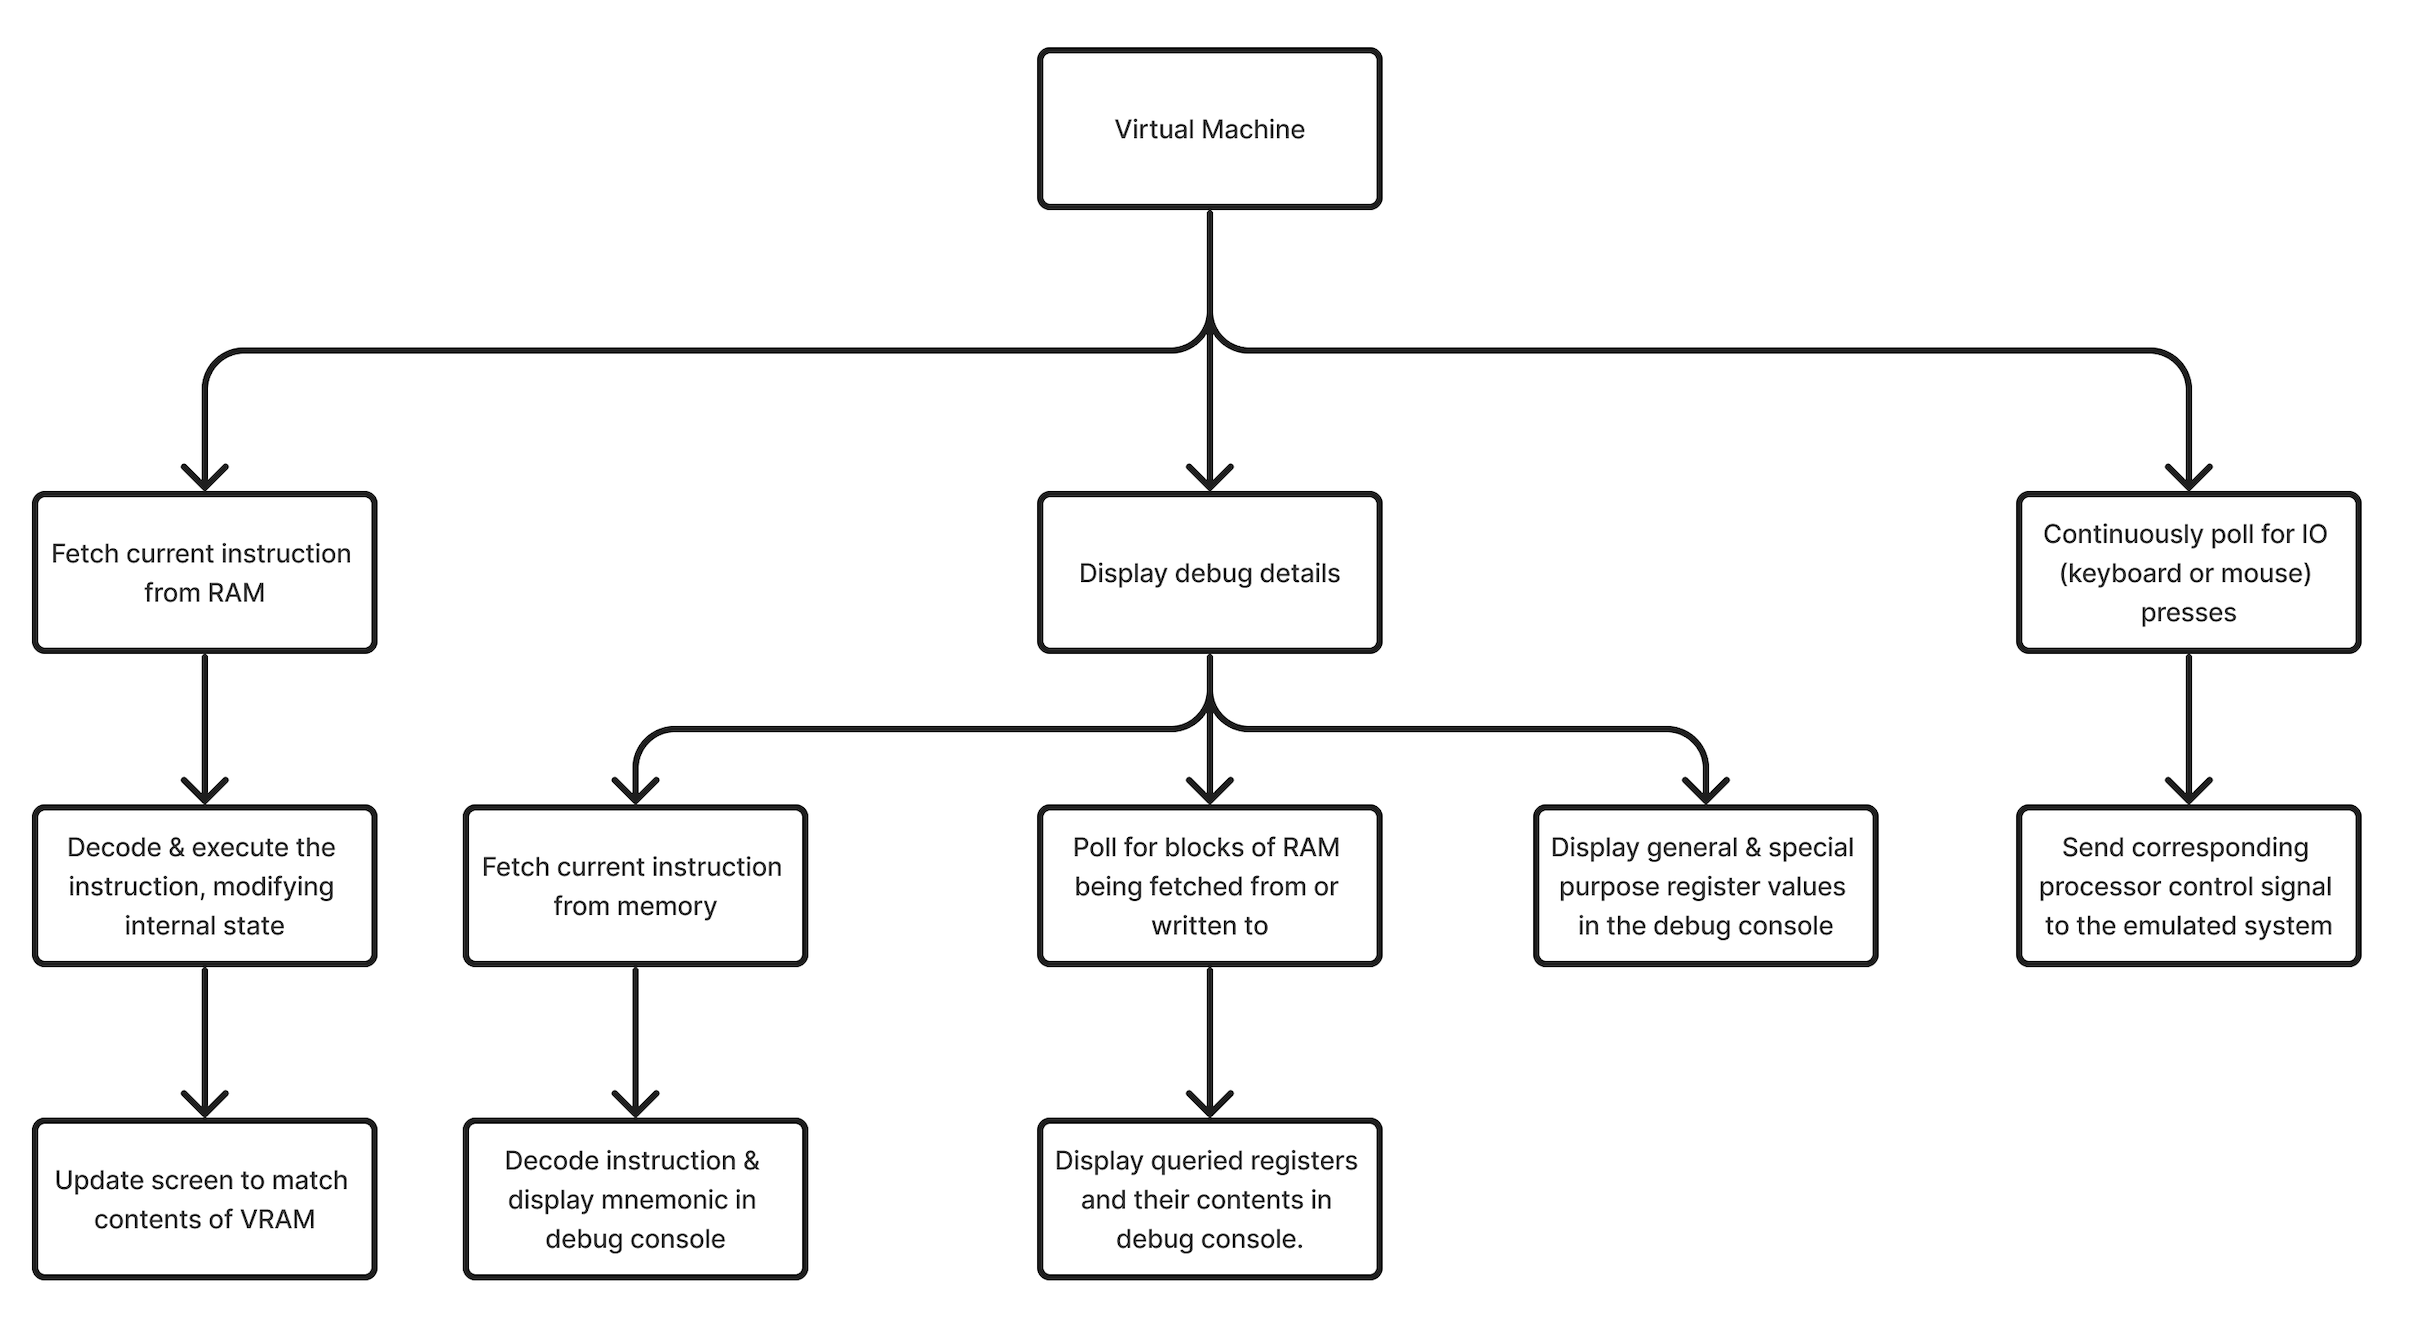
\includegraphics[width=13cm]{Screenshot 2024-07-23 at 13.51.25.png}
}

\bigskip

\begin{multicols}{2}[\columnsep-0.5em] 
    The assembler consists of a single pipeline for transforming ASCII assembly programs into binary machine code. The files are loaded into the interpreter which stores their contents in a string. The contents are then tokenised by a lexer into a list of objects representing the foundational elements of the program (e.g. STRING, BRACE, NUMBER) and parsed into a sequence of assembly language instructions. These instructions are translated into binary machine code according to the instruction set architecture (defined in \ref{sec:MachineCodeEncoding}) which is then written to a file and stored on the users computer.


    \columnbreak

    \shadowbox{
        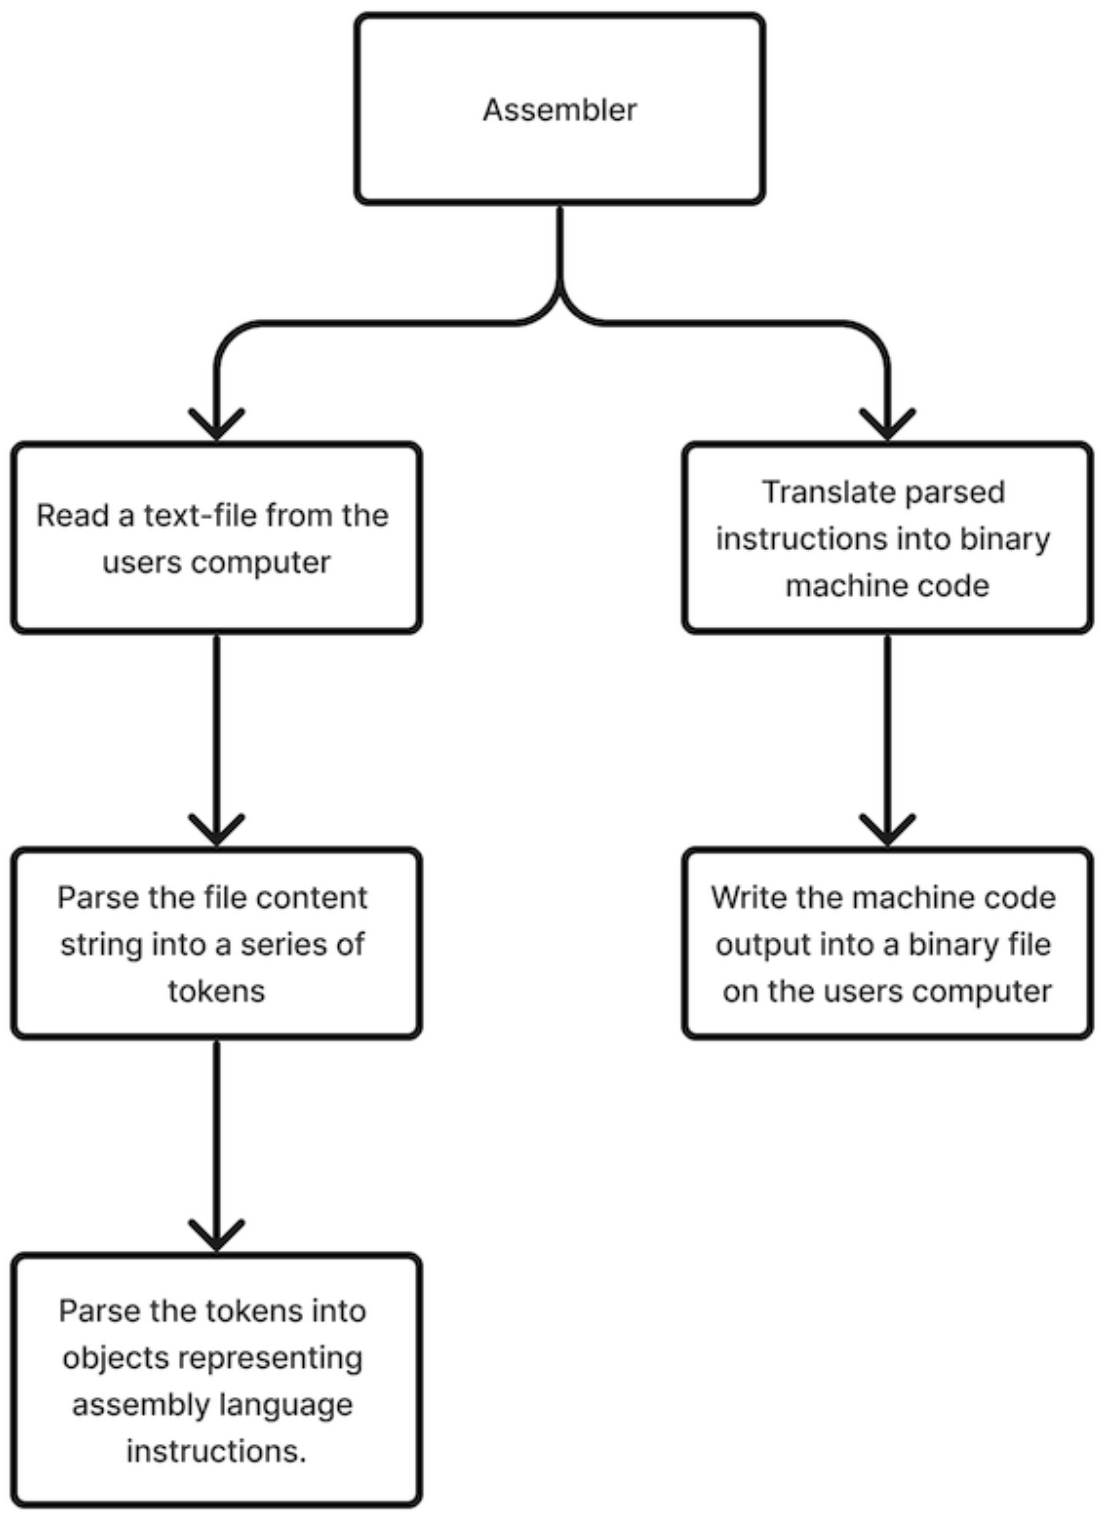
\includegraphics[width=5cm]{Screenshot 2024-07-23 at 12.47.14.png}
    }

\end{multicols}


\begin{wrapfigure}[13]{r}{8.5cm}
\shadowbox{
    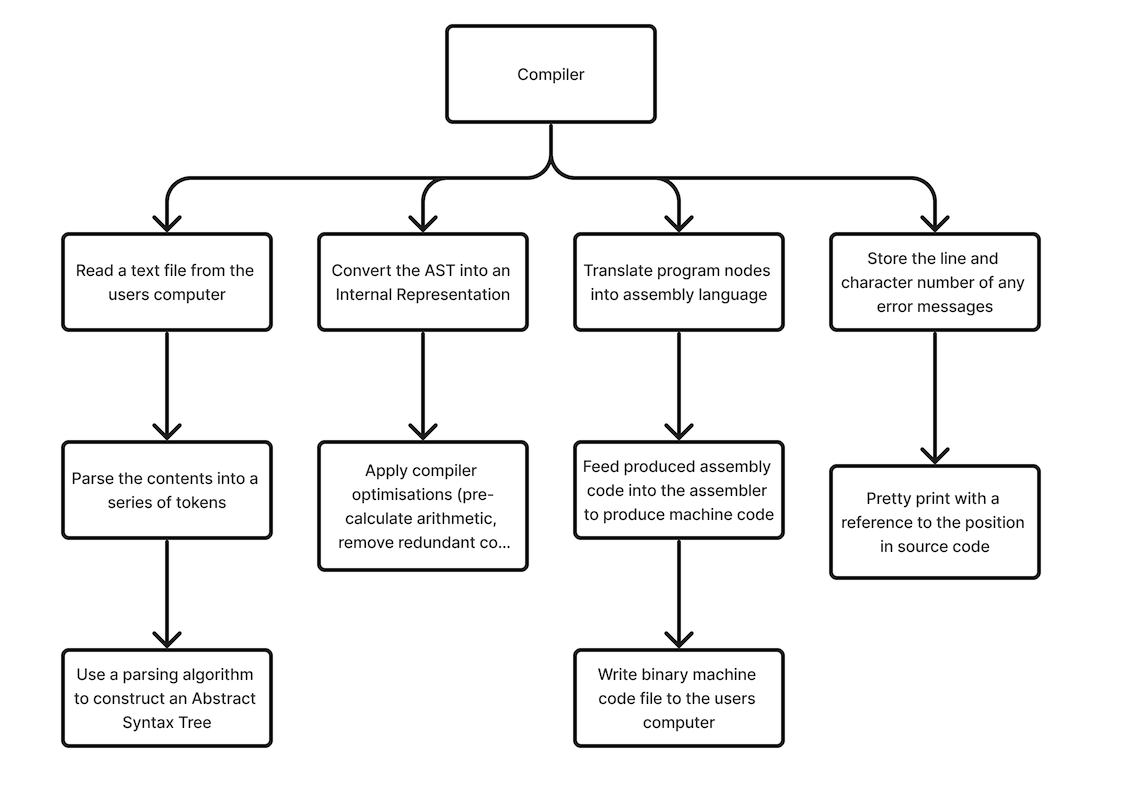
\includegraphics[width=8cm]{Screenshot 2024-06-24 at 19.30.50.png}
}
\end{wrapfigure}

\begin{samepage}

Much like the assembler, the compiler takes an ASCII program, converts it into tokens and parses it into an Abstract Syntax Tree (AST) representing the structure and order of operations of the program. This AST is converted into an internal representation (IR) designed to help easily locate potential optimisations in the source code (e.g. pre-calculating arithmetic or removing redundant code), these optimisations are made and the IR is converted into an intermediate assembly language due to the presence of high level optimisations such as labels and macro-instructions. Finally, this assembly code is inserted into the assembler and the produced machine code is stored as a file on the users computer. 

\end{samepage}

\bigskip

\subsection{Component Design}
\subsubsection{Instruction Set Architecture}

\subsubsubsection{Computer Architecture}
Having to balance simplicity with convenience dictated the final design decisions for this computers CPU architecture.  There is 64Kb of memory (65,526 memory locations) specified by 16-bit addresses, requiring a 16-bit Program Counter (PC). The clock speed for the CPU runs at 600Hz. Each instruction is 32-bits, meaning two processor cycles are required to fetch an instruction and store the high and low words in the Current Instruction Register (CIR). 

I decided on 32 16-bit general purpose registers, any two of which can be inputs to the ALU, which itself has two outputs - a 16 bit result which can be written to a register or memory depending on the instruction, and a 1 bit zero bit which is set when the result of the calculation is 0.

There are a number of special purpose registers, which, by convention are dedicated an address in memory, one for the stack pointer (SP) and another for the sound timer (ST). There is no dedicated stack and is instead allocated a downwards growing section of memory. The stack stores register values and return addresses when calling functions, however since the instruction set contains no \texttt{call} or \texttt{ret} instructions, this must be performed manually by the programmer. Each cycle the sound timer is non-zero, the computer produces a sound and decrements ST, allowing the length of the noise to be specified.

\needspace{100pt}

\subsubsubsection{Arithmetic and Logic Unit}

\begin{wrapfigure}[10]{r}{6.5cm}
    \shadowbox{
        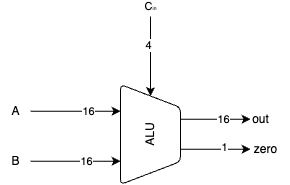
\includegraphics[width=6cm]{ALU schema.png}
    }
\end{wrapfigure}

The core of any instruction set is the Arithmetic Logic Unit (ALU) so I began by designing an interface for that. I decided on 2 16-bit inputs to the ALU, which can either take register values, or for an Ri-type instruction, the value of the 16-bit immediate field. There are 4 ALU control bits into the ALU, whcih dictate the operation to be performed. The first two control bits negate their respective inputs, and the second two determine the arithmetic or logical operation to perform. Combinations of these ALU control bits can produce a variety of different operations, all of which are detailed in the table below. (\cite{EOCS})

\bigskip

\begin{center}
    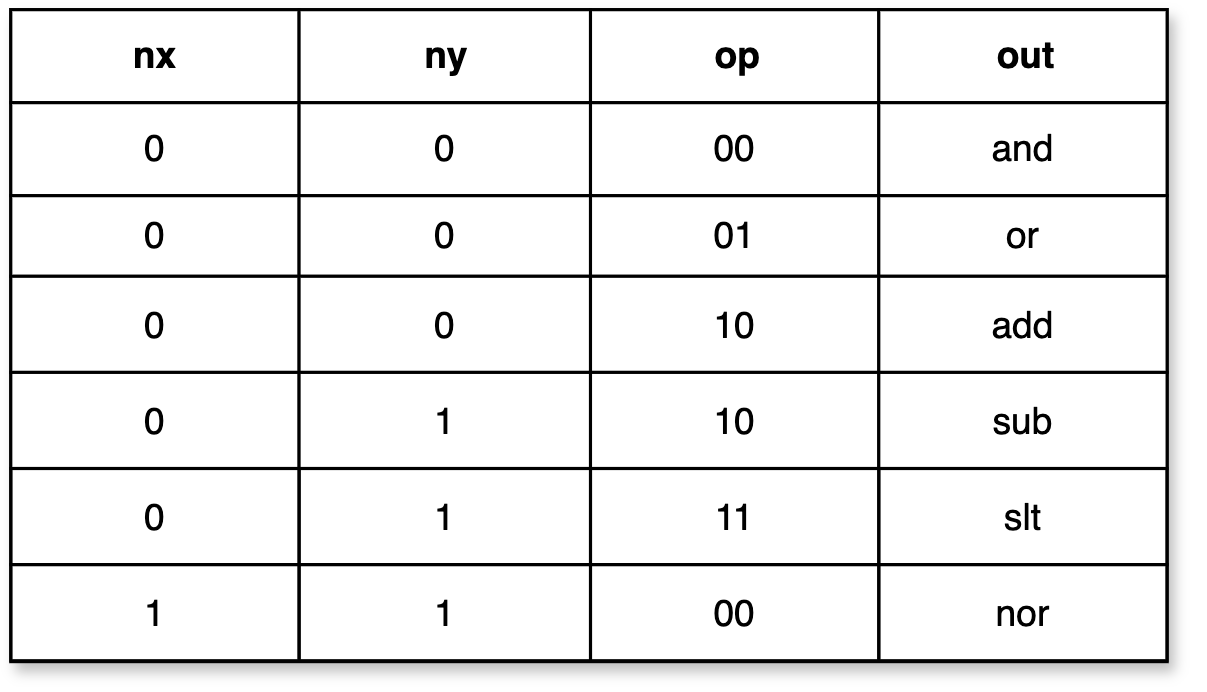
\includegraphics[width=8cm]{Screenshot 2024-08-29 at 19.34.16.png}
\end{center}

\subsubsubsection{Assembly Language}

I decided to use a MIPS instruction set architecture, minimising the number of instructions supported by the processor. I settled on 3 instruction types: R-type instructions (performing ALU operations on register values), I-type instructions (operations involving both registers and immediate fields), and J-type instructions (unconditional, absolute jumps to locations in memory). From these 3 types, the following instruction set can be constructed, demonstrated with a program to multiple two numbers stored in memory. (\texttt{'[]'} are used to indicate a memory address):

\begin{lstlisting}[language=C]
R-type: add, sub, and, or, nor, slt, sll, slr
I-type: addi, andi, ori, lw, sw, bge, bne
J-type: jmp

// multiply the numbers in memory address 0xb000 and 0xb001, and write the answer to 0xb002
li r31, 0xb000 // pointer to the start of data memory

lw r1, 0($r31)
lw r2, 1($r31)

.loop
    // if r2 is 0, break
    li r0, 0
    beq r0, r2, [.store]

    add r1, r1, r1

    addi r2, r2, -1

    jmp [.loop]

.store
    sw r1, 2($r31)
\end{lstlisting}

\subsubsubsection{Machine Code Encoding}
\label{sec:MachineCodeEncoding}
Below is the breakdown of how R/I/J type instructions are represented in binary, broken down into their respective fields. All instructions have a 4-bit opcode which dictates the type of instruction (and consequentially which of 4 encoding types should be used when decoding the instruction). For the purpose of machine code, L and Ri type instructions are encoded with the same fields.

\begin{itemize}
    \item \texttt{00-xx}: R-type instructions \textit{to perform operations between two registers}
        \begin{itemize}
            \item \texttt{5-bits rs}: the first of two input registers to the ALU.
            \item \texttt{5-bits rt}: the second of two input registers to the ALU.
            \item \texttt{5-bits rd}: the register in  which to store the result of the operation.
            \item \texttt{4-bits func}: the control bits determining the ALU operation.
        \end{itemize}
    \item \texttt{01-xx}: Ri-type instructions \textit{(to perform operations between a register and immediate value)}
        \begin{itemize}
            \item \texttt{5-bits rs}: the first of two input registers to the ALU.
            \item \texttt{5-bits rt}: the second of two input registers to the ALU.
            \item \texttt{16-bits immediate}: the data used as the second ALU input.
        \end{itemize}
    \item \texttt{10-xx}: L-type instructions \textit{(to load/store words from memory)}
        \begin{itemize}
            \item \texttt{5-bits rs}: the register containing the base offset for calculating memory addresses.
            \item \texttt{5-bits rt}: the register to store/read data from/into memory.
            \item \texttt{16-bits immediate}: the offset from the base address for the calculating memory addresses.
        \end{itemize}
    \item \texttt{11-xx}: J-type instructions \textit{(to jump to an address in memory)}
        \begin{itemize}
            \item \texttt{5-bits rs}: the register containing the memory address to branch to in RAM.
            \item \texttt{5-bits rt}: the register to store the return address of the jump.
            \item \texttt{16-bits immediate}: the address to branch to in RAM
        \end{itemize}
\end{itemize}
 
\bigskip

\begin{center}
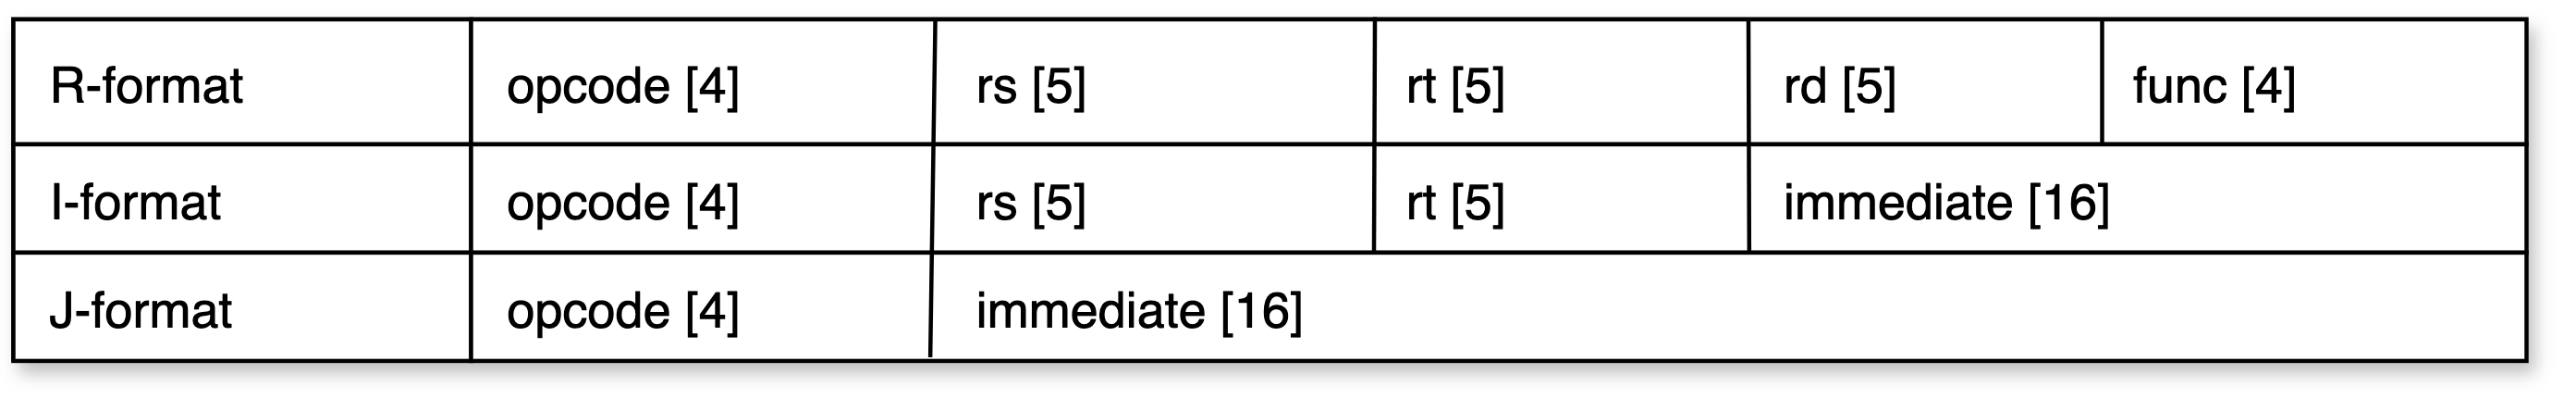
\includegraphics[width=14cm]{Screenshot 2024-08-29 at 22.34.18.png}
\end{center}

\bigskip

Next to each assembly instruction below is its machine code encoding, showing the relationship between the assembly language operands and the encoding fields. 

\begin{lstlisting}
addi $r5, $r0, 14      // 0110 00000 00101 00000000 00001110
lw $r4, 10($r30)       // 1000 11110 00100 00000000 00001010


slt $r0, $r1, $r2z     // 0000 00001 00010 00000 0111 
bne $r0, $r4, [0xb020] // 1101 00000 00100 10110000 00100000
jmp [0x8080]           // 1111 10000000 10000000
\end{lstlisting}

Since each instruction is 32-bits and contains two words, an instruction must be stored across two memory locations. Little-endian and Big-endian are different standards for storing data across multiple bytes, for little endian - the LSB of the instruction is stored in the first memory location and the MSB in the second, vise versa for big endian. The modern standard has become little-endian encoding, and is what I will use in this project. Hence, the instruction \texttt{0110110000000101 0000000000001110} would be stored in memory as:

\begin{lstlisting}
    [0]: 0000000000001110
    [1]: 0110110000000101 
\end{lstlisting}

\subsection{Virtual Machine}
The virtual machine should act as an interpreter, initialising a virtual processor - with an interface mimicking the registers, memory, and clock of the hardware descriptor. It needs to load a binary program cartridge into an array of bytes represening the computers memory, and steps through it word by word, decoding each instruction encountered and carrying out the subsequent operations accordingly. The data structure representing the processor will look as follows:

\begin{lstlisting}
STRUCT lion
    SIGNED WORD[65535] memory
    SIGNED WORD[32] registers
    UNSIGNED WORD pc
    UNSIGNED WORD elapsed_cycles;
ENDSTRUCT
\end{lstlisting}

The processor has $2^{16}$ different 16-bit memory locations, both this and the 32 general-purpose registers can be  represented by an array of signed words. The program counter must remain unsigned however, as its sole purpose is to point to locations in memory. The elapsed cycles field will be used to keep track of the number of cycles each instruction takes to execute - and to tell the emulator how long to wait for to maintain correct clock timing.

\subsubsection{Algorithms}

\subsubsubsection{Fetch-Execute Cycle}
The virtual machines primary directive is to simulate the fetch-decode execute cycle of the processor. This involves fetching an instruction from memory, incrementing the program counter, and then depending on the opcode of the fetched instruction, executing logic to handle that instruction. The \texttt{elapsed\_cycles} field on the struct can be used to keep a record of the time the program should wait after each instruction to maintain consistancy with the clock speed of the processor. The basic structure for the fetch-execute cycle procedure should look as follows:

\begin{lstlisting}
PROCEDURE FETCH_EXECUTE()
    READ BINARY CARTRIDGE INTO MEMORY ARRAY

    WHILE PROCESSOR IS RUNNING
        IF CPU CYCLES BACKLOG IS EMPTY
            FETCH INSTRUCTION 
            INCREMENT PC

            MATCH ON INSTRUCTION OPCODE 
                R: 
                    MAP func FIELD TO OPERATION 
                    FETCH REGISTER VALUES 
                    PERFORM OPERATION ON REGISTERS 
                    STORE RESULT IN REGISTER 
                    SET CPU CYCLES BACKLOG 
                LW:
                    FETCH REGISTER VALUE
                    SUM ADDRESS AND REGISTER
                    SET ADDRESS TO RESULT
                    FETCH VALUE FROM MEMORY LOCATION
                    STORE THE RESULT IN REGISTER
                    SET CPU CYCLES BACKLOG
                JAL:
                    STORE PC VALUE IN REGISTER
                    SET PC TO IMMEDIATE FIELD
                    SET CPU CYCLES BACKLOG
        ELSE 
            DECREASE CPU CYCLES BACKLOG

        WAIT CLOCK CYCLE
ENDPROCEDURE
\end{lstlisting}

First the words from \texttt{memory[pc]} and \texttt{memory[pc+1]} must be fetched and stored together in a 32-bit current instruction register. From here, the 4-bit opcode should be extracted and used to determine how the instruction is executed. Each instruction will take multiple clock cycles to execute, and the field \texttt{elapsed\_cycles} on the \texttt{lion struct} is used to keep track of this, after each instruction is executed, the processor should wait for \texttt{elapsed\_cycles} clock cycles before proceeding to the next. 

Since each instruction is 32-bits, instructions span 2 memory locations and are stored according to the little endian convention, where the least significant byte is stored in the first location. Below is the pseudocode for fetch-execute cycle algorithm: 

\begin{lstlisting}
PROCEDURE FETCH_EXECUTE 
    READ_FILE_INTO_MEOMRY()

    WHILE (NOT hlt) DO 
        // only begin the next instruction cycle once the previous has finished executing
        IF (elapsed_cycles == 0) THEN 
            // the first byte in memory is the LSB and the second the MSB
            // binary shift the MSB 16 places to make room for the LSB
            UNSIGNED WORD cir = (memory[pc+1] << 16) | memory[pc]
            pc += 2

            EXECUTE_INSTRUCTION(cir)
        ELSE 
            elapsed_cycles -= 1
        ENDIF

        WAIT 1/CLOCK_SPEED
    ENDWHILE
ENDPROCEDURE

PROCEDURE EXECUTE_INSTRUCTION(u32 instruction)
    NIBBLE opcode = instruction & 0xF000 
    MATCH (opcode) 
        CASE 0x0000: 
            UNSIGNED BYTE rs = instruction[4:9]
            UNSIGNED BYTE rt = instruction[10:15]
            UNSIGNED BYTE rd = instruction[16:21]
            UNSIGNED BYTE func = instruction[22:26]

            SIGNED WORD OP() = MAP[func] 
            registers[rd] = OP(rs, rt)
            elapsed_cycles = 4
            BREAK

        CASE 0100: // lw rt, i16($rs)
            SIGNED WORD offset = instruction[16:]
            UNSIGNED BYTE rs = instruction[4:9]
            UNSIGNED BYTE rt = instruction[10:15]

            UNSIGNED WORD address = offset + registers[rs]
            registers[rt] = memory[address]
            elapsed_cycles = 4
            BREAK;

        CASE 0x1111: // jal i16
            UNSIGNED BYTE rt = instruction[10:15]
            registers[rt] = pc
            pc = instruction[16:]
            elapsed_cycles = 3
            BREAK
    END
END
\end{lstlisting}

\subsubsubsection{Reading a Binary File}
The virtual machine needs to be able to load a binary program from a file on the users computer into the processors memory array. This should default to the first address in memory since the pc (program counter) should point to the first instruction and the computer lacks a bootloader. The algorithm should open the file on the users computer from the filename provided in the CLI arguments, and reads it through two bytes at a time, loading each word into the processors memory array - until the end of the file has been reached.

\begin{lstlisting}
PROCEDURE READ_FILE_INTO_MEMORY() 
    IF (LEN(ARGS) <= 1) THEN 
        THROW "Missing filename argument"
    ENDIF 

    STRING filename = ARGS[1] // get cartridge filename from cli arguments

    // open the file and read in the first word (2 bytes)
    FILE file = OPEN(filename)

    // since the file size is in bytes, and iterating through words, SIZE(file)/2
    FOR (WORD address = 0; address < SIZE(file)/2; address ++) DO
        memory[address] = READ_WORD(file)
    ENDFOR
ENDPROCEDURE
\end{lstlisting}


\subsection{Assembler}
The assembler takes in an assembly program as a text file, and outputs the corresponding binary machine code. It consists of three parts: a lexical analysis of the text that produces an array of textual elements (e.g. NUMBER, LABEL, COLON); a parser that combines these program tokens into a sequence of instructions; and finally a compiler to synthesise machine code instructions. The broad pipeline for the assembler should look like the following:

\begin{lstlisting}
PROCEDURE assemble() 
    READ TEXT FILE INTO STRING
    lex()     // COMPILE PROGRAM STRING INTO A TOKEN ARRAY
    parse()   // COMBINE TOKENS INTO A SERIES OF INSTRUCTIONS
    compile() // CONVERT INSTRUCTIONS INTO MACHINE CODE
ENDPROCEDURE

PROCEDURE lex() 
    ITERATE THROUGH THE PROGRAM CHARACTER BY CHARACTER
    CREATE A VECTOR OF TOKENS
    MATCH CHARACTER 
        FOR A SINGLE CHARACTER TOKEN e.g. ('(', '$',',')
        APPEND THE TOKEN TO THE VECTOR

        FOR A MULTI CHARACTER TOKEN e.g. numbers
        CREATE A NUMBER STRING
        WHILE character IS A NUMBER 
            APPEND character TO NUMBER STRING 
        ENDWHILE 
        PARSE NUMBER STRING TO INTEGER 
        APPEND TOKEN TO THE VECTOR
    ENDMATCH

    APPEND EOF TOKEN TO VECTOR
ENDPROCEDURE

PROCEDURE parse()

ENDPROCEDURE
\end{lstlisting}

\subsubsection{Data Structures}

\subsubsubsection{Token}
I need a token data structure to represent the program elements in the lexical stage of the assembler, it needs to be addressed in a uniform manner regardless of the type, and since different tokens can take different arguments - this logic needs to be split into an enum. The token struct should contain the position of the token (both start and end position since tokens can vary in length), and this can be used to generate error messages that point to the particular location in the file in which the error occured. 

\begin{lstlisting}
STRUCT TOKEN 
    TOKEN_TYPE t_type
    UNSIGNED INTEGER s_pos 
    UNSIGNED INTEGER e_pos 
ENDSTRUCT 

ENUM TOKEN_TYPE
    NUMBER(i16),
    LABEL(String),
    REGISTER(String),
    LPAREN,
    RPAREN,
    LSQUARE,
    RSQUARE
    DOLLAR,
    COMMA,
    DOT,
    ADD 
    BNE, 
    JAL
ENDENUM
\end{lstlisting}

\subsubsubsection{SyntaxError}
One of the objectives for this project (Objective 2.6) was the production of relevant error messages - pointing out the position in source code in which they occur. I decided on the format below for syntax errors. 

\begin{lstlisting}
SyntaxError: invalid character '%', line: 2
lw $r0, 10(%r0)
           ^
\end{lstlisting}

For this: two things are required, the error message itself, and the position of the error (start and end position). The program string itself instead of being included in the error can be passed as a parameter when displaying the message, and from this, the display method should be able to reference the line and character(s) on which the error occured.

\begin{lstlisting}
STRUCT SYNTAX_ERROR
    STRING msg
    UNSIGNED INTEGER s_pos 
    UNSIGNED INTEGER e_pos
ENDSTRUCT
\end{lstlisting}

The algorithm to display syntax errors should convert the s\_pos and e\_pos variables into a line number and column tuple, (initially an index in the 1 dimensional program string). It should then identify the column of the line in which the error occurs and print a carrat under that character. Since s\_pos and e\_pos refer to indexes in the program string, to gather the line number and column in which they occur: after iterating through the string line by line and decrementing the variables by the number of characters on each line, when the variables are less than the length of the subsequent line, the (line, col) position of the error has been found.

\begin{lstlisting}
PROCEDURE DISPLAY_SYNTAX_ERROR(program: STRING)
    SPLIT PROGRAM INTO LINES
    ITERATE THROUGH EACH LINE 
        DECREMENT s_pos and e_pos BY EACH LINE LENGTH 

        WHEN s_pos < THIS LINE LENGTH 
        SET (s_line, s_col) TUPLE

        WHEN e_pos < THIS LINE LENGTH
        SET (e_line, e_col) TUPLE

    PRINT msg, "line: ", line
    PRINT line 
    PRINT " " * (s_col-1) + "^"*(e_col-s_col) + " " * LEN(line) - e_col
ENDPROCEDURE
\end{lstlisting}

\subsubsection{Algorithms}

\subsubsubsection{Lexical Analysis}
